\documentclass[a4paper,12pt]{article}
\usepackage[utf8]{inputenc}
\usepackage[T1]{fontenc}
\usepackage[romanian]{babel}
\usepackage{amsmath, amssymb}
\usepackage{graphicx}
\usepackage{hyperref}
\usepackage[a4paper, margin=2cm]{geometry}

\title{Raport AP1}
\author{Chiriac Laura-Florina}
\date{Ianuarie 2025}

\begin{document}

\maketitle

\section{Descrierea Problemei}
\subsection{Contextul}
Acest proiect are ca scop predicția soldului total (diferența dintre producție și consumul de energie electrică) din Sistemul Energetic Național (SEN) al României pentru luna decembrie 2024. Datele utilizate sunt obținute de pe platforma Transelectrica SEN Grafic și includ informații despre consumul și producția de energie defalcate pe diverse surse.

\subsection{Scopul Proiectului}
Obiectivul este de a implementa două modele de învățare automată, adaptate pentru regresie: arborele de decizie ID3 și clasificarea Bayesiană. Modelele trebuie să fie evaluate pe baza performanțelor obținute (ex. RMSE, MAE).

\section{Analiza Problemei}
\subsection{Descrierea Setului de Date}
Setul de date conține următoarele coloane principale:
\begin{itemize}
    \item \textbf{Data}: Timpul specific al înregistrării.
    \item \textbf{Consum[MW]}: Consumul total de energie electrică.
    \item \textbf{Producție[MW]}: Producția totală de energie.
    \item Diverse surse de producție, inclusiv \textbf{Carbune[MW]}, \textbf{Hidrocarburi[MW]}, \textbf{Ape[MW]}, \textbf{Nuclear[MW]}, \textbf{Eolian[MW]}, \textbf{Foto[MW]}, \textbf{Biomasă[MW]}.
    \item \textbf{Sold[MW]}: Diferența între producție și consum.
\end{itemize}

Datele pentru luna decembrie au fost excluse din antrenare și utilizate exclusiv pentru testare.

\subsection{Preprocesarea Setului de Date}
\begin{itemize}
    \item Datele pentru luna decembrie au fost excluse din antrenare și utilizate exclusiv pentru testare.
    \item Au fost adăugate caracteristici suplimentare prin agregare: \\
    \textbf{Intermittent[MW]}: Sumă între producția eoliană și solară. \\
    \textbf{Constant[MW]}: Sumă între producția nucleară, pe bază de cărbune și hidrocarburi.
    \item Pentru Bayes, datele continue au fost discretizate în 5 intervale.
\end{itemize}

\subsection{Explorarea Relațiilor}
Am observat corelații între \textbf{Consum}, \textbf{Producție} și \textbf{Sold}. Sursele intermitente (eolian, solar) contribuie semnificativ la variațiile în \textbf{Sold}, în timp ce sursele constante (nuclear, hidro) oferă stabilitate.

\subsection{Adaptarea Algoritmilor}
\subsection*{Adaptări pentru ID3}
Arborele de decizie ID3 a fost adaptat pentru regresie folosind criteriul \textbf{squared error} și discretizarea intervalelor pentru predicții mai precise. Modelul a fost optimizat folosind \textbf{GridSearchCV} cu hiperparametri precum:
\begin{itemize}
    \item \textbf{max\_depth}: Adâncimea maximă a arborelui.
    \item \textbf{min\_samples\_split}: Numărul minim de eșantioane necesare pentru a împărți un nod.
    \item \textbf{min\_samples\_leaf}: Numărul minim de eșantioane la o frunză.
\end{itemize}

\subsection*{Adaptări pentru Clasificarea Bayesiană}
\begin{itemize}
    \item Am discretizat variabilele continue pentru compatibilitate cu clasificarea bayesiană.
    \item Am folosit Gaussian Naive Bayes și am aplicat categorizarea soldului în clase (Very Low, Low, Medium, High, Very High).
\end{itemize}

\subsection{Rezultate și Evaluarea Modelelor}
Evaluarea modelelor a fost realizată folosind următoarele metrici:
\begin{itemize}
    \item \textbf{RMSE (Root Mean Squared Error)}: $\sqrt{\frac{1}{n}\sum_{i=1}^{n}(y_i - \hat{y}_i)^2}$
    \item \textbf{MAE (Mean Absolute Error)}: $\frac{1}{n}\sum_{i=1}^{n}|y_i - \hat{y}_i|$
    \item \textbf{Accuracy}: $\frac{\text{Numărul de predicții corecte}}{\text{Numărul total de predicții}}$
\end{itemize}
Acestea au fost integrate în scriptul final \texttt{main.py}, unde se prezic datele din decembrie 2024, pentru a evalua rezultatele.

\section{Justificarea Abordării}
\subsection{ID3 și Clasificarea Bayesiană}
Am optat pentru algoritmul ID3 și clasificarea bayesiană, deoarece ambele metode sunt eficiente în tratarea problemelor de regresie pe baza datelor istorice. ID3, folosind arbori de decizie, oferă transparență și ușurință în înțelegerea deciziilor, evidențiind corelațiile dintre variabile. Clasificarea bayesiană, pe de altă parte, furnizează un cadru probabilistic care gestionează variabilitatea și incertitudinea datelor, fiind potrivită pentru estimarea valorilor continue.

\subsection{Logica programului}
Logica programului implică câteva etape care au fost luate în calcul în cadrul tuturor algoritmilor încercați: Preprocesarea datelor prin agregare pe zile (în script-urile \texttt{daily\_data.csv} și \texttt{daily\_december\_2024.csv}), iar apoi prin eliminarea valorilor lipsă și filtrare, apoi transformarea Sold în variabilă categorică (cu valori High, Low, etc.) și la final aplicarea modelului ID3 sau Bayes pe acest set de date. \\

\subsubsection{aggregate\_train\_data.py}
Scriptul combină și prelucrează datele brute din fișierele pentru 2022 și 2023(\texttt{Grafic\_SEN\_2022.xlsx} și \texttt{Grafic\_SEN\_2023.xlsx} din folderul data), convertind coloana Data în format datetime și valorile numerice relevante. Apoi, agregă datele la nivel zilnic, calculând sumele pentru consum, producție și tipurile de energie. Adaugă o coloană Sold[MW], care reprezintă diferența dintre producție și consum. Rezultatele sunt salvate într-un fișier CSV pentru utilizare ulterioară, numit \texttt{daily\_data.csv)}:


\begin{figure}
    \centering
    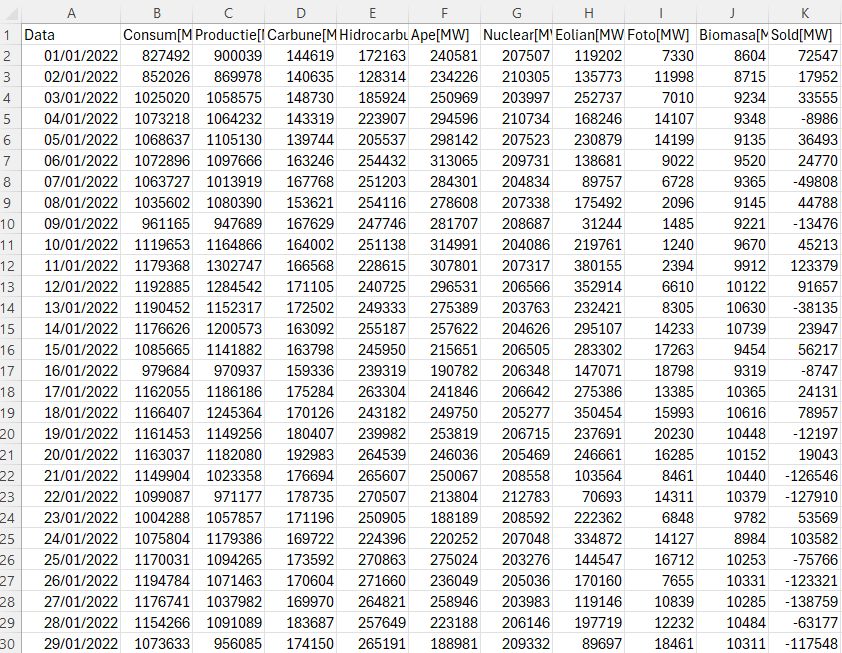
\includegraphics[width=0.8\textwidth]{img1.png}
    \caption{Date energetice (agregate) - 2022-2023}
    \label{fig:date zilnice 2022-2023}
\end{figure}

\subsubsection{aggregate\_test\_data.py}
Scriptul prelucrează datele de test din fișierul pentru \textbf{decembrie 2024} (\texttt{december\_2024.py}), convertind coloana Data în format datetime și transformând valorile numerice relevante. Agregă datele la nivel zilnic, calculând sumele pentru consum, producție și sursele de energie. Adaugă o coloană Sold[MW], reprezentând diferența dintre producție și consum. Rezultatele sunt salvate într-un fișier CSV numit \texttt{daily\_december\_2024.py}pentru utilizare mai ușoară, în special pentru compararea cu rezultatul predicției:

\begin{figure}
    \centering
    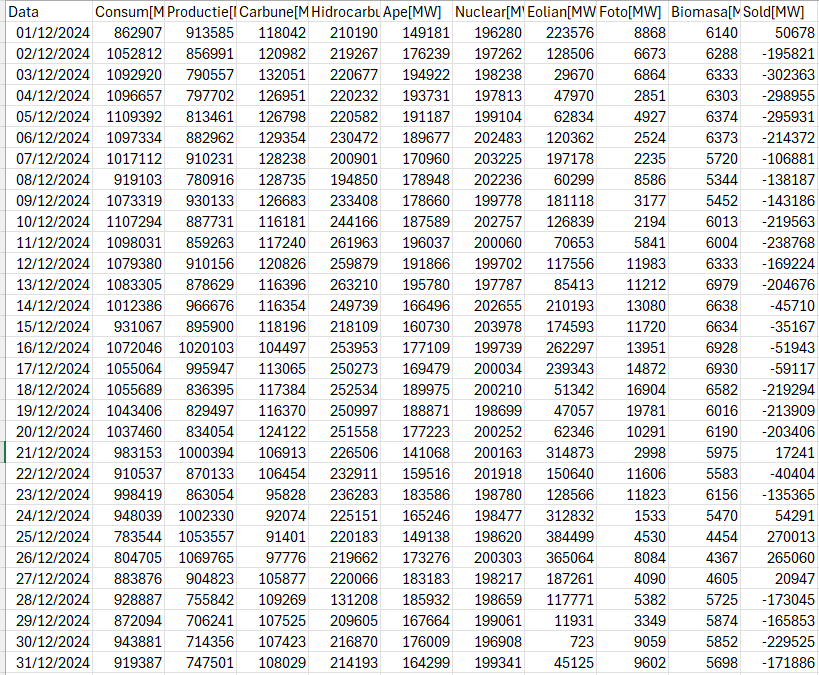
\includegraphics[width=0.8\textwidth]{img2.png}
    \caption{Date energetice (agregate) - decembrie 2024}
    \label{fig:date zilnice decembrie 2024}
\end{figure}

\subsubsection{id3.py, id3\_2.py, id3\_3.py}
Variațiile ID3 reprezintă încercările făcute pentru a găsi cea mai bună soluție pentru ID3. În general, toate cele 3 încercări au rezultate destul de bune, asemănătoare, și toate au un algoritm similar. Diferențele dintre ele sunt nu foarte multe, dar relevante:
\begin{itemize}
    \item Pentru \texttt{id3.py} și \texttt{id3\_2.py}: Preprocesarea datelor este similară, dar fără a adăuga coloane suplimentare de tipul Intermittent[MW] și Constant[MW]. Aceastea folosesc un set de caracteristici mai larg pentru a modela datele de intrare.
    \item Pentru \texttt{id3\_2.py}: Datele lipsă sunt completate cu valoarea 0, ceea ce poate duce la unele erori dacă 0 nu este un indicator adecvat pentru datele lipsă. De altfel, fără adăugarea coloanelor suplimentare și cu acest tip de abordare, deși face ce fac și ceilalți algoritmi ID3, acesta este cel mai neoptim.
    \item Pentru \texttt{id3\_3.py}: Deși această variantă a ID3 este destul de potrivită, deoarece date sunt preprocesate mai bine, singurul lucru care diferențiază această variantă de cea găsită ca fiind cea mai bună este ajustarea hiperparametrilor pentru ID3.
\end{itemize}

\begin{figure}[ht!]
    \centering
    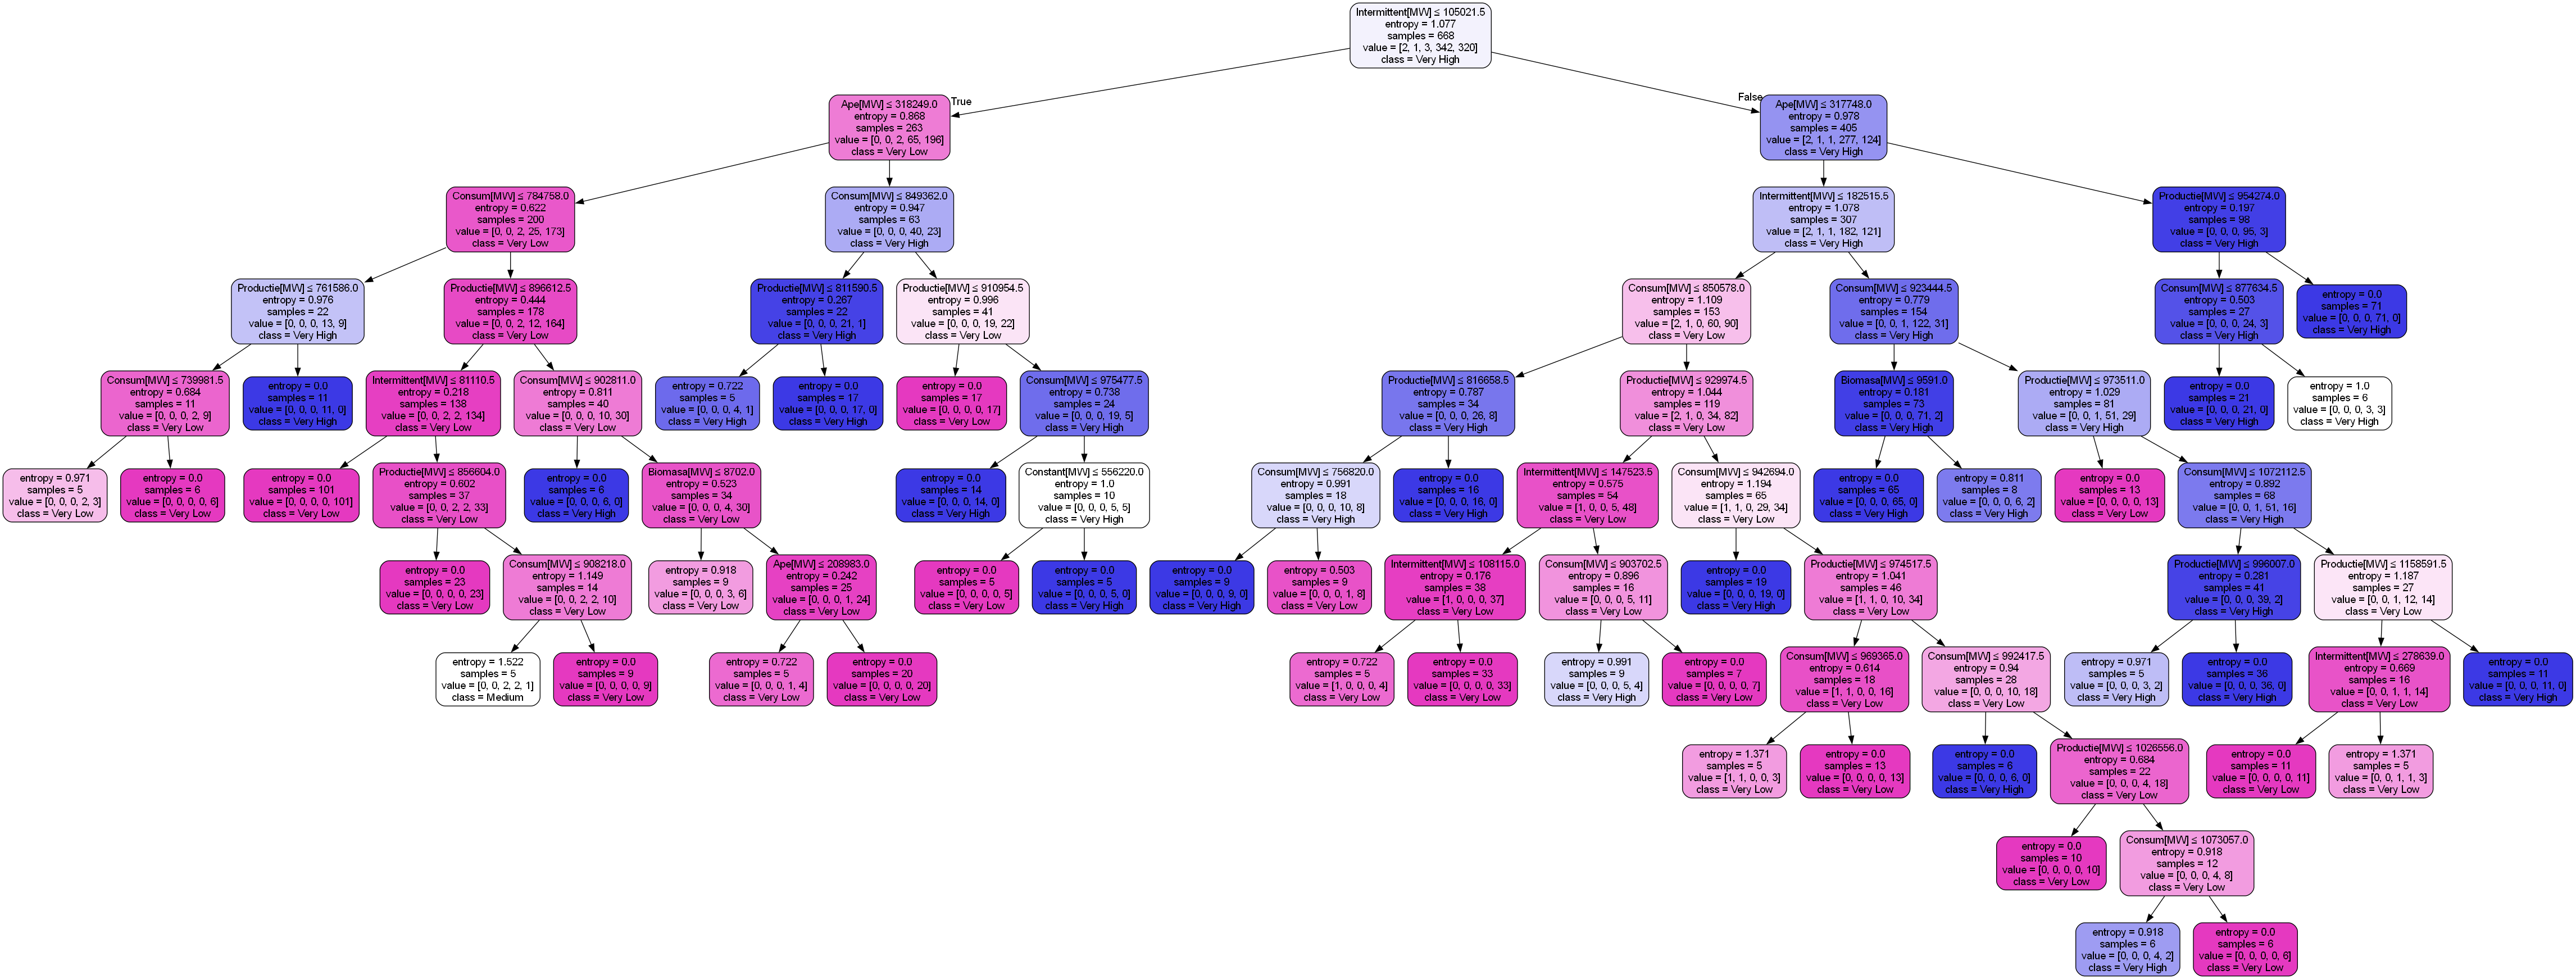
\includegraphics[width=1\textwidth, height=7cm]{tree.png}
    \caption{Vizualizarea arborelui de decizie ID3.}
\end{figure}

\subsubsection{main.py}
Scriptul \texttt{main.py} este scriptul principal folosit ca să prezic datele din decembrie 2024. Diferența dintre acesta și a doua cea mai performantă versiune a ID3 este faptul că au fost ajustați hiperparametrii de la GridSearch pentru o căutare mai performantă a celui mai bun model și o performanță per total puțin mai mare a algoritmului. Pe lângă aceasta, fișierul pune datele prezise în 2 moduri: cel al clasificatorului ID3 în funcție de categoriile Sold-ului și varianta cu regresie, într-un fișier numit \texttt{predictions\_december\_2024.csv} (din folderul data):

\begin{figure}
    \centering
    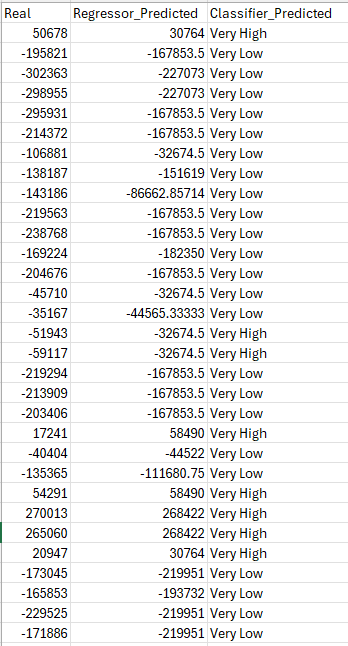
\includegraphics[width=0.5\textwidth]{img3.png}
    \caption{Predicții Sold[MW] - Decembrie 2024 (Clasificare)}
    \label{fig:predictii2024_clasificare}
\end{figure}

\section{Prezentarea Rezultatelor}
Pentru evaluarea performanței algoritmilor adaptați (ID3 și clasificarea Bayesiană), au fost calculate metrice relevante, cum ar fi eroarea medie pătratică (RMSE), eroarea absolută medie (MAE) și acuratețea (Accuracy). Aceste valori oferă o perspectivă detaliată asupra calității predicțiilor pentru fiecare metodă și variantă de algoritm ID3 utilizată.

\subsection{Rezultate principale}
Tabelul de mai jos sumarizează performanțele algoritmilor: \\
\begin{table}[!ht]
\centering
\begin{tabular}{|l|c|c|c|c|}
\hline
\textbf{Metrică}       & \textbf{ID3}      & \textbf{Bayes}   & \textbf{ID3 (var2)} & \textbf{ID3 (var3)} \\ \hline
\textbf{RMSE}          & 45,380.64         & 171,402.49       & 38,587.34           & 45,333.71           \\ \hline
\textbf{MAE}           & 35,742.62         & 142,876.26       & 1,488,982,909.83    & 35,498.48           \\ \hline
\textbf{Accuracy (\%)}      & 93.55             & 61.29            & 90.32               
& 93.55                \\ \hline
\end{tabular}
\caption{Rezultatele algoritmilor pentru metricele RMSE, MAE și Acuratețe.}
\label{tab:rezultate_algoritmi}
\end{table}

\subsection{Observații și interpretări}
\begin{itemize}
    \item \textbf{ID3:}
    \begin{itemize}
        \item Algoritmul de bază ID3 a obținut valori foarte bune pentru acuratețe (\textbf{93.55\%}) și a menținut un nivel scăzut al erorii (MAE: \textbf{35,742.62}, RMSE: \textbf{45,380.64}).
        \item Variantele sale adaptate (\textit{var2} și \textit{var3}) au arătat performanțe similare, cu \textit{ID3\_var2} înregistrând cea mai mică valoare RMSE (\textbf{38,587.34}), ceea ce indică o mai bună aproximare a valorilor reale, dar o valoare extrem de mare a MSE și o acuratețe mai mică. 
        \item Astfel, pe baza datelor obținute am ales prima variantă a lui ID3 care are, în urma testelor efectuate, cea mai mare acuratețe (la mică diferență de a treia variantă) și a menținut și un nivel scăzut al erorii.
    \end{itemize}
    \item \textbf{Clasificarea Bayesiană:}
    \begin{itemize}
        \item Algoritmul Bayesian a înregistrat o acuratețe semnificativ mai mică (\textbf{61.29\%}) și valori ridicate ale erorilor (RMSE: \textbf{171,402.49}, MAE: \textbf{142,876.26}). Acest rezultat sugerează dificultăți în gestionarea complexității relațiilor dintre variabile.
    \end{itemize}
\end{itemize}

\subsection{Concluzii intermediare}
Algoritmul ID3 standard și variantele sale sunt mai bine adaptate pentru această problemă, oferind o combinație echilibrată între precizie și stabilitate. Clasificarea Bayesiană este mai puțin performantă în acest context, având dificultăți în a surprinde relațiile complexe dintre variabilele de intrare.

\subsection{Observații finale}
\begin{itemize}
    \item \textbf{Distribuția predicțiilor}: Majoritatea valorilor reale și prezise indică solduri energetice negative semnificative, clasificate ca „Very Low,” ceea ce sugerează un deficit energetic constant în decembrie. Exemple includ valorile reale -302,363 și -298,955, predictibile ca „Very Low” de ambele metode.
    \item \textbf{Abaterea între metode}: Algoritmul Bayesian oferă predicții mai moderate față de regressor. De exemplu, pentru valoarea reală -214,372, predicția Bayes este 127,415 (pozitivă), în timp ce regresorul prezice -167,853.5 (negativă), evidențiind o discrepanță semnificativă.
    \item \textbf{Corectitudinea predicțiilor ridicate}: Pentru zilele cu sold pozitiv (e.g., 27 și 28, cu valori reale 270,013 și 265,060), ambele metode prezic valori \textbf{„Very High”} indicând o bună acuratețe în identificarea excedentelor.
    \item \textbf{Tendințe generale:}
        \begin{itemize}
            \item Valorile reale negative sunt, în general, asociate cu clasificarea \textit{Very Low}, iar valorile pozitive mari cu \textit{Very High}, ceea ce indică o capacitate bună de diferențiere a modelului de clasificare între cele două clase extreme. \\
            \item Predicțiile regresorului arată o acuratețe mai mare decât cele ale modelului Bayesian, în special pentru valori pozitive mari. \\
        \end{itemize}
\end{itemize}

Aceste observații sugerează că algoritmul ID3 în varianta regresor are o performanță mai consistentă în comparație cu clasificarea Bayesiană, în special pentru valori pozitive mari și extreme. Totuși, ajustările suplimentare ale hiperparametrilor ar putea îmbunătăți performanța modelului Bayesian.

\section{Concluzii}
În cadrul acestui proiect, utilizarea algoritmilor ID3 și clasificarea bayesiană pentru regresie a evidențiat avantajele și limitările fiecărei metode. ID3 s-a dovedit eficient în identificarea relațiilor între variabilele de intrare, oferind predicții precise pentru majoritatea cazurilor. În schimb, clasificarea bayesiană a prezentat o performanță mai slabă în scenarii cu variabilitate ridicată, dar a demonstrat robustețe în gestionarea datelor zgomotoase.

\subsection*{Ce am învățat:}
\begin{itemize}
    \item Algoritmul ID3 adaptat pentru regresie oferă predicții precise pentru \textit{Sold[MW]}.
    \item Clasificarea bayesiană necesită o discretizare atentă pentru a concura cu ID3.
\end{itemize}

Codul curent (cel din main.py, ales ca fiind cel mai bun) reprezintă o variantă optimă deoarece:
\begin{itemize}
    \item Rezultatele obținute sunt semnificativ mai bune decât cele din încercările anterioare.
    \item Abordările folosite optimizează atât antrenarea, cât și interpretabilitatea modelelor.
\end{itemize}

\subsection*{Îmbunătățirea performanței} 
    Pentru îmbunătățirea performanței, pot fi explorate următoarele soluții:
\begin{itemize}
    \item Crearea de caracteristici suplimentare pe baza datelor existente.
    \item Utilizarea altor metode de adaptare pentru regresie.
    \item Integrarea unei metode de reducere a dimensiunii sau de selecție a caracteristicilor pentru a simplifica arborii generați de ID3.
    \item Ajustarea distribuțiilor și a ipotezelor utilizate în clasificarea bayesiană pentru a îmbunătăți acuratețea în scenarii complexe.
    \item Combinarea celor două metode într-o abordare hibridă, folosind punctele forte ale fiecărei tehnici pentru a crește acuratețea și robustețea predicțiilor.
\end{itemize}

\section*{Cod și Soluție Practică}
Codul sursă, împreună cu explicațiile, este disponibil în repozitoriul GitHub: \url{https://github.com/LauraC360/AP1_ML}

\end{document}